Before we start with the basics of the Finite Difference method, we should quickly recall the definition 
of the derivative of a function. 

\begin{center}
{\sl 
The derivative of a function $y=f(x)$ of a variable $x$ is a measure of the rate at which the value $y$ 
of the function changes with respect to the change of the variable $x$. It is called "the derivative of $f$ 
with respect to $x$". If $x$ and $y$ are real numbers, and if the graph of $f$ is plotted against $x$, the derivative 
is the \underline{slope} of this graph at each point. 
}
\end{center}

\noindent There are two standard notations:
\begin{equation}
\frac{df}{dx}(x) \qquad \text{and} \qquad f'(x)
\end{equation}
The mathematical definition is\footnote{if the limit exists}:
\begin{equation}
\boxed{
f'(x)
=\lim_{h\rightarrow 0} \frac{f(x+h)-f(x)}{(x+h)-x} 
=\lim_{h\rightarrow 0} \frac{f(x+h)-f(x)}{h} 
}
\end{equation}
i.e., how much does the function grow between $x$ and $x+h$, divided by the length $h$.
On the following left plot the function is in green while the line joining the points
$x,f(x)$ and $x+h,f(x+h)$ is shown in purple. On the right figure we see that 
when $h$ becomes smaller and smaller this line does indeed get closer and closer 
to the real tangent line in brown.

\begin{center}
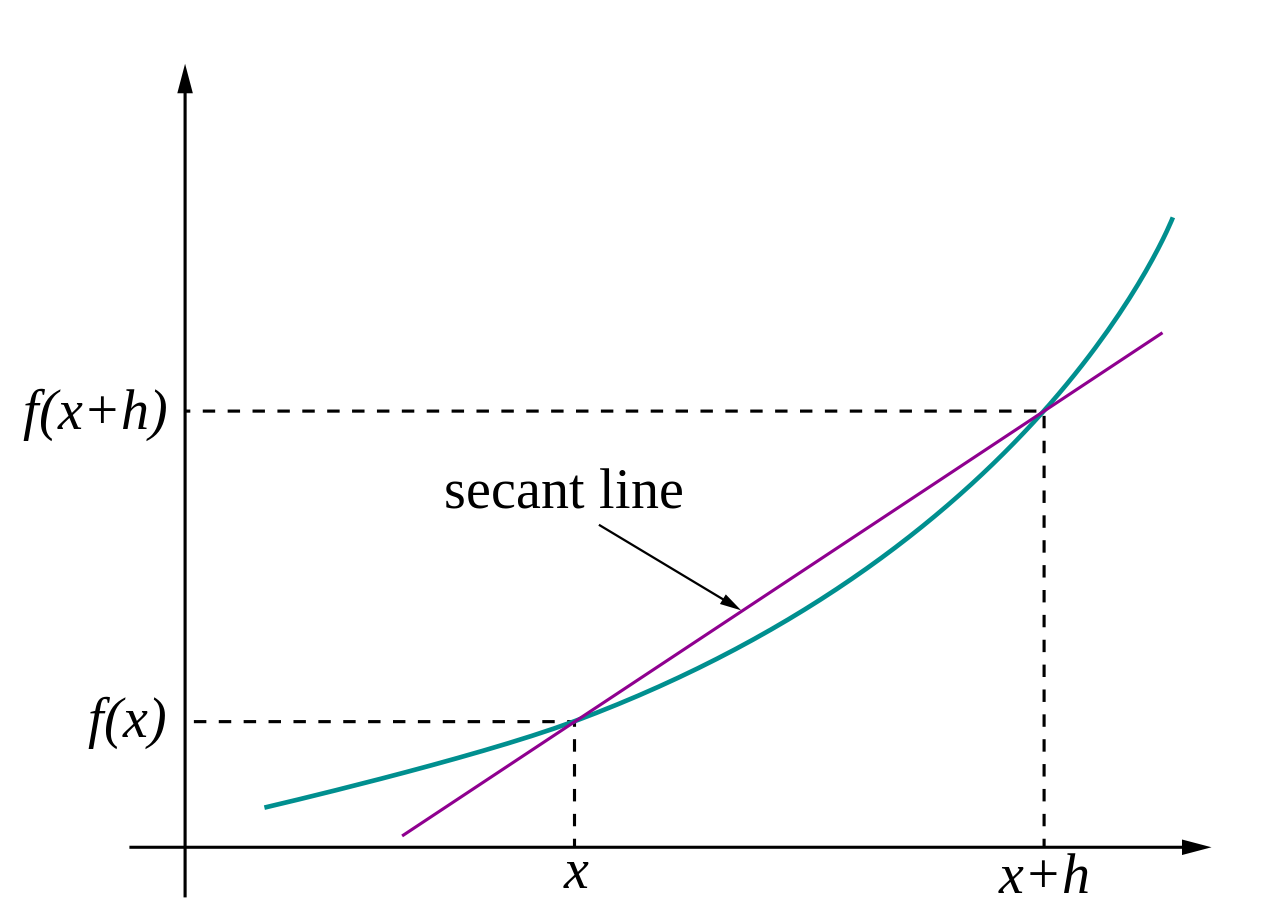
\includegraphics[width=7.4cm]{images/derivative/der2}
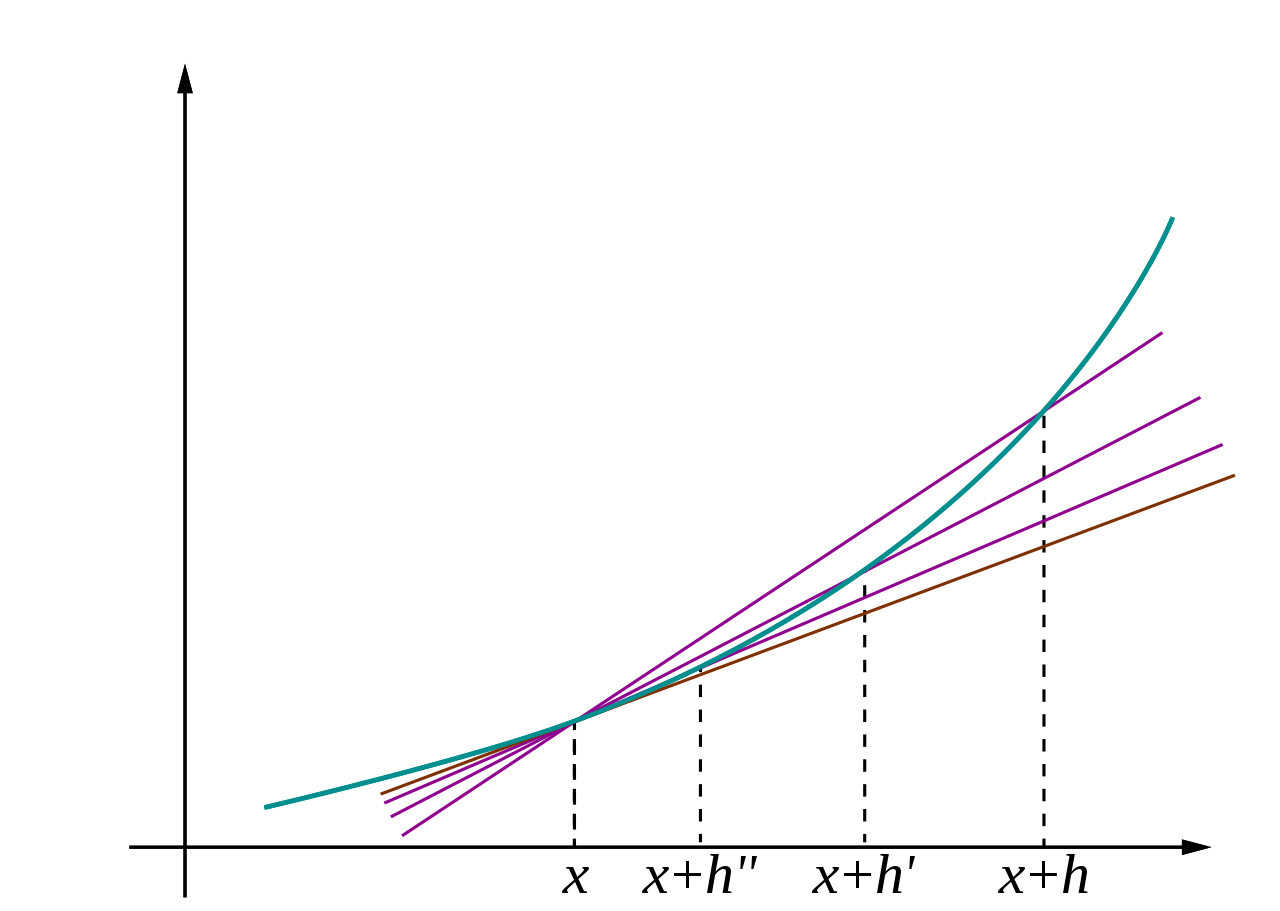
\includegraphics[width=7.4cm]{images/derivative/der1}\\
{\captionfont 
Left: The secant to curve $y=f(x)$ determined by points $(x,f(x))$ and $(x+h, f(x+h))$;
Right: The tangent line as limit of secants ($h''<h'<h$).
Taken from Wikipedia\footnote{\url{https://en.wikipedia.org/wiki/Derivative}}.
}
\end{center}

\noindent Also, one can rewrite the formula above as
\begin{equation}
f(x+h) \simeq f(x) +  f'(x) h
\end{equation}
which is in fact the beginning of the Taylor expansion of the function:
\begin{equation}
f(x+h) \simeq f(x) +  f'(x) h + \frac{1}{2!} f''(x) h^2 + \dots 
\end{equation}
We will see in what follows that the Taylor expansion and the concept of derivation is 
central in the Finite Difference method. 

